	\chapter{Kravspecifikation}
	
		\section{Systembeskrivelse}
		Der ønskes lavet en applikation som får folk til at lege mere med farveskift af lyset på deres Philips Hue pærer.
		Applikationen skal kunne skifte lyset instant, gemme temaer man kan sætte i gang på givende tidspunkter, måske hvis en speciel playliste bliver sat på. Man skal kunne bruge applikationen til at betjene flere forskellige pærer.
		Der vil blive udviklet en applikation som snakker op til et API, som er udstedet af et andet firma, for at se at dette faktisk er en reel arbejdsmodel man kan bruge i hverdagen.
		Dette sker ved at der i applikationen skal snakkes op til Philips Hue API for at kunne tilgå pærerne.
		\newline
		
		\subsection{Use Case}
		\begin{itemize}
			\item Bruger kommer hjem
			\item Bruger tænder sin Philips Hue pærer
			\item Bruger sætter en bestemt playliste på sine højtaler
			\item Pæren skifter til det brugerdefinerede tema som er valgt til denne playliste i sin ”Shine My Room” applikation
			\item Brugeren stopper musikken
			\item Pæren skifter til normalvisning \newline
		\end{itemize}
	
		\subsection{Designovervejelser}
		Billedet herunder beskriver vores første design tanker til applikationen
		\begin{figure}[H]
			\centering
			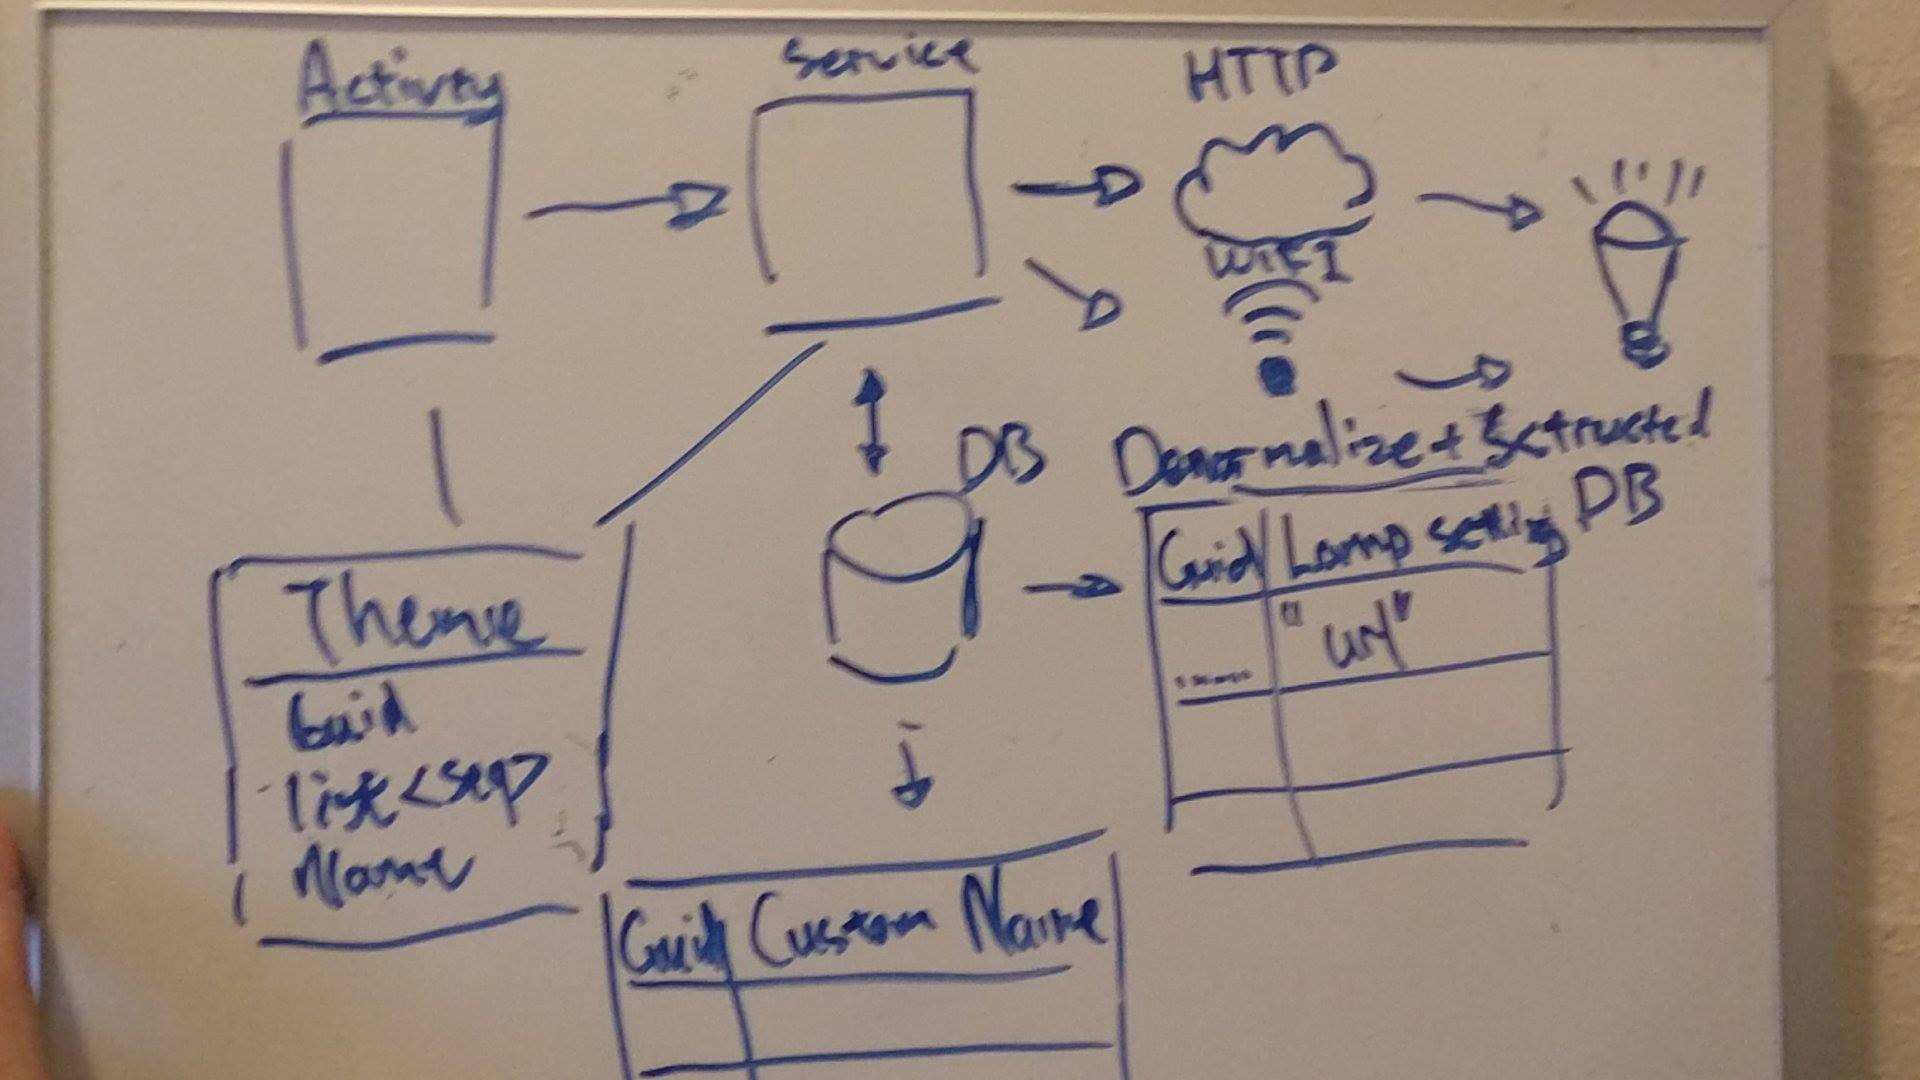
\includegraphics[width=0.6\linewidth]{Kravspecifikation/Designovervejelser}
			\caption{Oversigt over systemet}
			\label{fig:Designovervejelser}
		\end{figure}
		\newpage
	
		\subsection{Riskovervejelser}
		Med udgangspunktet fra applikationens side, vi der være en risk i forhold til:
		\begin{itemize}
			\item Hvor meget plads vores data vil tage
			\item Hvor meget strøm det tager for brugeren. 
			\item Kommer vi til at bruge meget internet når vi sender en sekvens af API kald til lamperne, og hvor stort et problem det bliver at sørge for at det bliver i en sekvensilt rækkefølge.
			\item Hvordan vi intercepter lyd output fra mobilen og evt. skærm output. \newline
		\end{itemize}	
		
		
		\section{Work plan}
		
		
	